% ! TEX root = ../story.tex

\chapter{Descrierea aplicației}

Aplicația servește la gestionarea unei biblioteci, în relația cu cititorii,
oferind roluri speciale pentru clienți din mediul academic.

%%%%%%%%%%%%%%%%%%%%%%%%%%%%%%%%%%%%%%%%%%%%%%%%%%%%%%%%%%%%%%%%%%%%%% 
\section{Utilizatori și atribute}
\label{sec:util-atr}
\index{utilizatori}
\index{atribute}

Utilizatorii aplicației, identificați prin IP-uri specifice sînt:
\begin{itemize}
\item \textbf{Administratori} ai bazei de date;
\item \textbf{Personal educațional} (\texttt{EDU});
\item \textbf{Cititori} din afara mediului educațional (\texttt{NEDU});
\item \textbf{Bibliotecari};
\item \textbf{Cititori înregistrați, dar neabonați} (\texttt{RESTUL}).
\end{itemize}

Considerăm că studenții și profesorii fac parte din personalul educațional
(Edu), statut pe care trebuie să-l verifice periodic. De asemenea, un
cititor oarecare poate deveni Edu în timp, dacă adaugă verificarea.

%%%%%%%%%%%%%%%%%%%%%%%%%%%%%%%%%%%%%%%%%%%%%%%%%%%%%%%%%%%%%%%%%%%%%% 
\section{Procesele din aplicație}
\label{sec:procese}
\index{procese}

\begin{enumerate}[(P1)]
\item Vizualizarea cărților în stoc;
\item Vizualizarea bibliotecarilor, cu specializările lor;
\item Adăugarea unei cărți;
\item Adăugarea unui cititor;
\item Adăugarea unui abonat Edu;
\item Înregistrarea unui cont public;
\item Actualizarea stocului unor cărți;
\item Verificarea statutului Edu;
\item Administrarea abonamentului;
\item Vizualizarea cărților de o anumită specializare;
\item Vizualizarea revistelor de o anumită specializare;
\item Adăugare reviste;
\item Administrare abonament revistă;
\item Administrare abonament la newsletter;
\item Împrumut carte;
\item Feedback bibliotecar.
\end{enumerate}

\index{procese!descompunere funcțională}
De exemplu, \textbf{descompunerea funcțională} a procesului (P14),
de administrare a abonamentului la o revistă, poate fi reprezentat ca în
figura \ref{fig:proc-abonare-rev}.

\begin{figure}[!htbp]
  \centering
  \usetikzlibrary{positioning}
  \usetikzlibrary{shapes.geometric}
  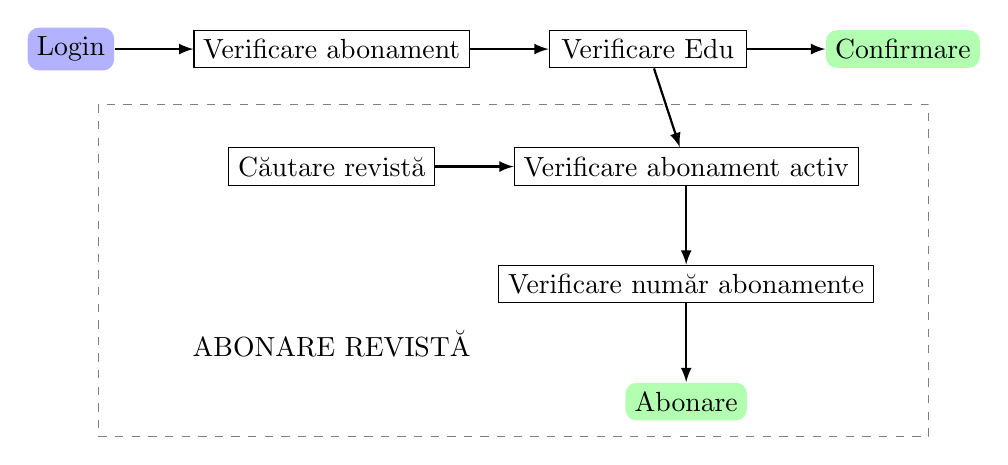
\begin{tikzpicture}[
    node distance=1cm,
    startstop/.style={rectangle,rounded corners,text centered,fill=blue!30},
    process/.style={rectangle,minimum width=2.5cm, draw=black},
    ok/.style={rectangle,rounded corners,text centered, fill=green!30},
    nob/.style={minimum width=2.5cm},
    arr/.style={thick,-latex}
    ]
    \node (login) [startstop] {Login};
    \node (vab) [process,right=of login] {Verificare abonament};
    \node (ved) [process,right=of vab] {Verificare Edu};
    \node (ok) [ok,right=of ved] {Confirmare};
    \draw[arr] (login) -- (vab);
    \draw[arr] (vab) -- (ved);
    \draw[arr] (ved) -- (ok);
    \draw [draw=black!50, below=of ved, xshift=1em,yshift=-2em,dashed] rectangle +(30em,-12em);
    \node (crev) [process,below=of vab] {Căutare revistă};
    \node (vaba) [process,right=of crev] {Verificare abonament activ};
    \node (vnab) [process,below=of vaba] {Verificare număr abonamente};
    \node (abo) [ok,below=of vnab] {Abonare};
    \node (abr) [nob,below=of crev,yshift=-2em] {ABONARE REVISTĂ};
    \draw[arr] (crev) -- (vaba);
    \draw[arr] (vaba) -- (vnab);
    \draw[arr] (vnab) -- (abo);
    \draw[arr] (ved) -- (vaba);
  \end{tikzpicture}
  \caption{Descompunerea funcțională a procesului de abonare la revistă}
  \label{fig:proc-abonare-rev}
\end{figure}

Similar, procesul (P9) de verificare a statutului Edu se poate reprezenta
ca în figura \ref{fig:verif-edu}.

\begin{figure}[!htbp]
  \centering
  \usetikzlibrary{positioning}
  \usetikzlibrary{shapes.geometric}
  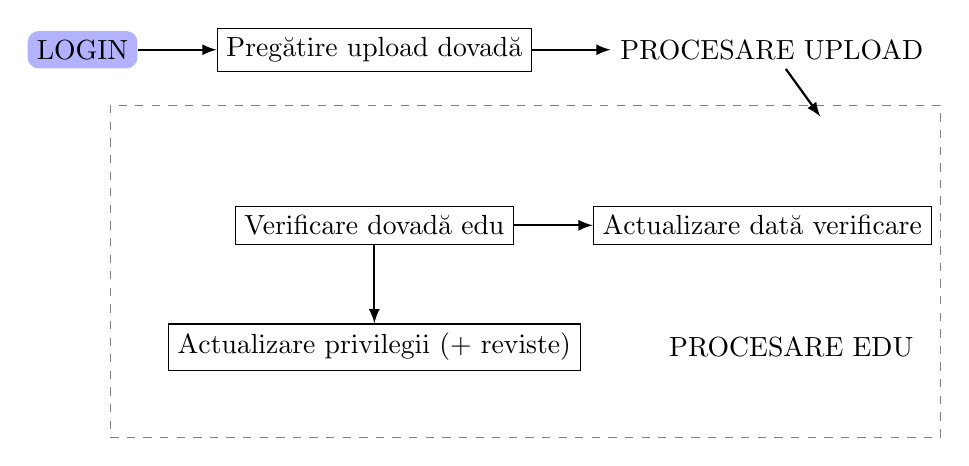
\begin{tikzpicture}[
    node distance=1cm,
    startstop/.style={rectangle,rounded corners,text centered,fill=blue!30},
    process/.style={rectangle,minimum width=2.5cm, draw=black},
    ok/.style={rectangle,rounded corners,text centered, fill=green!30},
    nob/.style={minimum width=2.5cm},
    arr/.style={thick,-latex}
    ]
    \node (login) [startstop] {LOGIN};
    \node (up) [process,right=of login] {Pregătire upload dovadă};
    \node (pu) [nob,right=of up] {PROCESARE UPLOAD};
    \draw [draw=black!50, below=of pu, xshift=1em,yshift=-2em,dashed] rectangle +(30em,-12em);
    \node (ved) [process, below=of up, yshift=-2em] {Verificare dovadă edu};
    \node (adv) [process, right=of ved] {Actualizare dată verificare};
    \node (actp) [process, below=of ved] {Actualizare privilegii (+ reviste)};
    \node (ped) [nob, right=of actp] {PROCESARE EDU};
    \draw[arr] (login) -- (up);
    \draw[arr] (up) -- (pu);
    \draw[arr] (pu) -- (9.37,-0.85);
    \draw[arr] (ved) -- (adv);
    \draw[arr] (ved) -- (actp);
  \end{tikzpicture}
  \caption{Descompunerea funcțională a procesului de verificare Edu}
  \label{fig:verif-edu}
\end{figure}

Și un ultim exemplu pe care îl prezentăm este acela al procesului (P16),
de scriere a feedback-ului pentru un bibliotecar. Descompunerea
funcțională este prezentată în figura \ref{fig:+fb}.

\begin{figure}[!htbp]
  \centering
  \usetikzlibrary{positioning}
  \usetikzlibrary{shapes.geometric}
  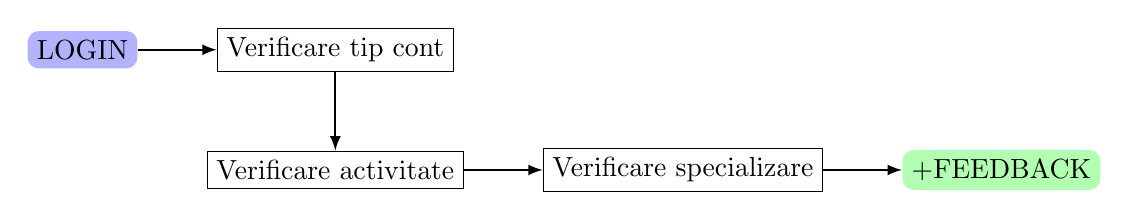
\begin{tikzpicture}[
    node distance=1cm,
    startstop/.style={rectangle,rounded corners,text centered,fill=blue!30},
    process/.style={rectangle,minimum width=2.5cm, draw=black},
    ok/.style={rectangle,rounded corners,text centered, fill=green!30},
    nob/.style={minimum width=2.5cm},
    arr/.style={thick,-latex}
    ]
    \node (login) [startstop] {LOGIN};
    \node (vc) [process,right=of login] {Verificare tip cont};
    \node (va) [process,below=of vc] {Verificare activitate};
    \node (vs) [process,right=of va] {Verificare specializare};
    \node (fd) [ok,right=of vs] {+FEEDBACK};
    \draw[arr] (login) -- (vc);
    \draw[arr] (vc) -- (va);
    \draw[arr] (va) -- (vs);
    \draw[arr] (vs) -- (fd);
  \end{tikzpicture}
  \caption{Descompunerea funcțională a procesului de adăugare feedback}
  \label{fig:+fb}
\end{figure}


%%%%%%%%%%%%%%%%%%%%%%%%%%%%%%%%%%%%%%%%%%%%%%%%%%%%%%%%%%%%%%%%%%%%%% 

\section{Matricea proces-utilizator}
\label{sec:matrice-pu}
\index{matrice!proces-utilizator}

\begin{center}
  \small
  \begin{tabular}{|l|c|c|c|c|c|c|c|c|c|c|c|c|c|c|c|c|}
    \hline
    & P1 & P2 & P3 & P4 & P5 & P6 & P7 & P8 & P9 & P10 & P11 & P12 & P13 & P14 & P15 & P16 \\
    \hline \hline
    Administrator & X & X & X & X & X & X & X & X & X & X & X & X & X & X & X & X \\
    \hline
    Edu & X & X & & & & & & X & X & X & X & & & X & X & X \\
    \hline
    NEdu & X & X & & & & & & X & X & X & & & & X & X & X \\
    \hline
    Bibliotecar & X & X & X & X & X & & & & X & X & X & X & X & X & & \\
    \hline
    Public & X & & & & & & & & & X & & & & X & & \\
    \hline
  \end{tabular}
\end{center}

%%%%%%%%%%%%%%%%%%%%%%%%%%%%%%%%%%%%%%%%%%%%%%%%%%%%%%%%%%%%%%%%%%%%%% 

\section{Entitățile și modelarea datelor}
\label{sec:ent-model}
\index{entități}
\index{modelarea datelor}

Biblioteca este un centru de împrumut care permite și abonamentul la reviste
pentru cei din mediul academic.

În bibliotecă se pot adăuga \emph{cărți} și \emph{reviste} de diverse
specializări, în funcție de contractele cu furnizorii. Fiecare
carte și revistă aparțin unei singure specializări.

Personalul Edu se poate abona și la reviste de specialitate, în baza
unei verificări actualizate. Ceilalți cititori cu abonament pot deveni
Edu printr-o verificare. Publicul larg poate doar să vadă stocul
de cărți, general sau pe specializări și să adauge cărțile dorite
în wishlist. Toți utilizatorii se pot abona la newsletter pentru a
afla cînd se actualizează stocul.

De asemenea, bibliotecarii sînt asociați specializărilor, fiind
responsabil de publicațiile dintr-o anumită specializare.

Cititorii abonați (\texttt{EDU} sau \texttt{NEDU}) pot lăsa feedback
bibliotecarilor cu care au lucrat anterior într-o anumită specializare.

Diagrama ER se poate prezenta ca în figura \ref{fig:erd}.

De menționat că toate relațiile M:M ($\infty : \infty$) vor fi rezolvate
cu \emph{tabelele asociative} \texttt{BIB\_SPEC}, \texttt{BIB\_CIT} și
\texttt{PUB\_CARTE}, listate la \S\ref{sec:scheme-rel}.

% \begin{verbatim}
%                            +-------------+
%                            | BIBLIOTECAR |
%                            +-------------+
%                             |           |
%                             |servește   |servește              +--------+ 
%                             | (M:M)     | (M:M)                | RESTUL |
%                             |           |                      +--------+
%   +---------+ se abonează +-----+    +------+                      |
%   | REVISTĂ |-------------| EDU |    | NEDU |                      |vizualizează
%   +---------+    (M:M)    +-----+    +------+                      |(M:M)
%        |                   |    \     |    \                       |
%        |                   |lasă \    |lasă \                      |
%        |                   |(1:M) \   |(1:M) \     (M:M)      +-------+
%        |                   |       \--|-------\---------------| CARTE |
%        |                  +------------+          împrumută   +-------+
%        |                  |  FEEDBACK  |                          |
%        |                  +------------+                          |
%        |se clasifică                                  se clasifică|
%        |după      (M:1)   +--------------+    (M:1)           după|
%        +------------------| SPECIALIZARE |------------------------+
%                           +--------------+
% \end{verbatim}


\newpage

\begin{landscape}
  \centering
  \begin{figure}[!h]
    \small
    \usetikzlibrary{positioning,shapes.multipart,shapes,cd,arrows.meta}
    \tikzset{basic/.style={
        draw,
        rectangle split,
        rectangle split parts=2,
        rectangle split part fill={blue!20,white},
        minimum width=3cm,
        % text width=2cm,
        align=center,
        font=\ttfamily
      },
      Diamond/.style={ rectangle, 
        draw, 
        shape aspect=3, 
        inner sep = 1pt,
        text centered,
        fill=orange!10!white,
        font=\itshape
      }}
    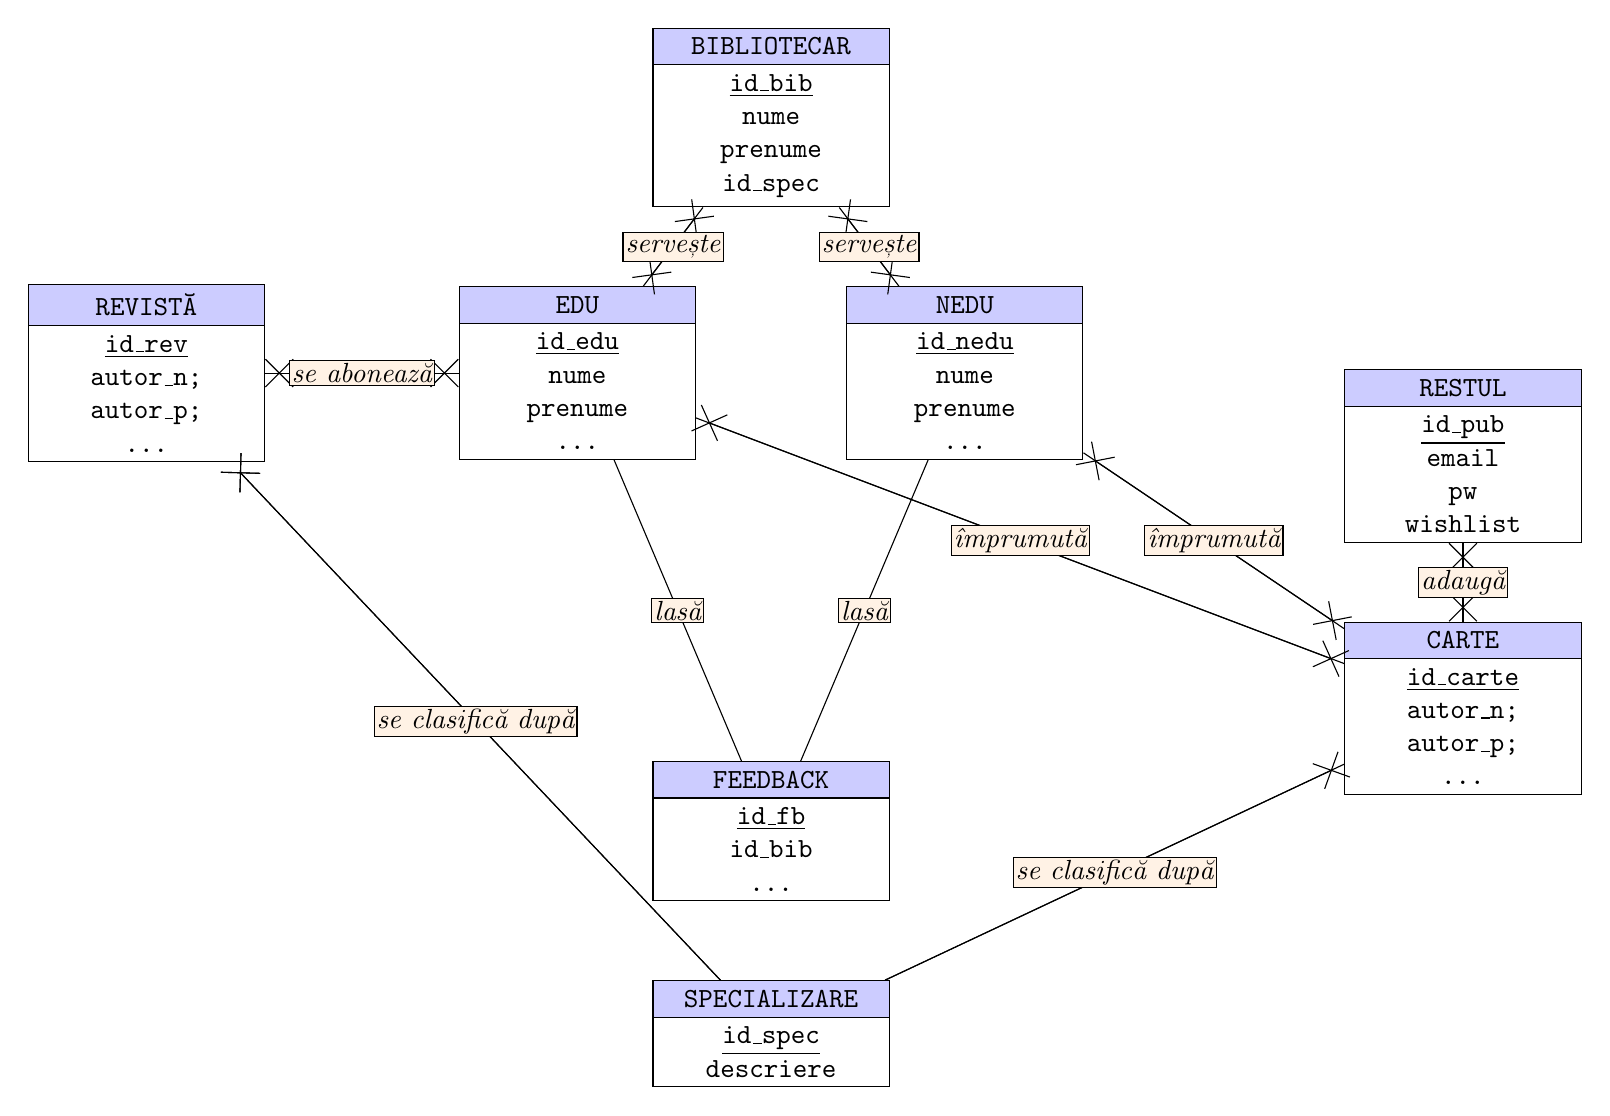
\begin{tikzpicture}
      \node[basic] (bib) {BIBLIOTECAR
        \nodepart{second}
        \underline{id\_bib}\\
        nume\\
        prenume\\
        id\_spec};
      \node[basic,below=of bib,xshift=-7em] (edu) {EDU
        \nodepart{second}
        \underline{id\_edu}\\
        nume\\
        prenume\\
        ...};
            \node[basic,below=of bib,xshift=7em] (nedu) {NEDU
        \nodepart{second}
        \underline{id\_nedu}\\
        nume\\
        prenume\\
        ...};
      \node[basic,below=of bib,xshift=25em,yshift=-3em] (pub) {RESTUL
        \nodepart{second}
        \underline{id\_pub}\\
        email\\
        pw \\
        wishlist};
      \node[basic,left=7em of edu] (rev) {REVISTĂ
        \nodepart{second}
        \underline{id\_rev}\\
        autor\_n;\\
        autor\_p;\\
        ...};
      \node[basic,below=of pub] (carte) {CARTE
        \nodepart{second}
        \underline{id\_carte}\\
        autor\_n;\\
        autor\_p;\\
        ...};
      \node[basic,below=20em of bib] (fdb) {FEEDBACK
        \nodepart{second}
        \underline{id\_fb}\\
        id\_bib\\
        ...};
      \node[basic,below=of fdb] (spec) {SPECIALIZARE
        \nodepart{second}
        \underline{id\_spec}\\
        descriere};
      \draw[-{Rays[n=4,length=5mm]}] (bib) -- (edu) node[midway,Diamond]{servește};
      \draw[-{Rays[n=4,length=5mm]}] (edu) -- (bib) node[midway,Diamond]{servește};
      \draw[-{Rays[n=4,length=5mm]}] (bib) -- (nedu) node[midway,Diamond]{servește};
      \draw[-{Rays[n=4,length=5mm]}] (nedu) -- (bib) node[midway,Diamond]{servește};
      \draw[-{Rays[n=4,length=5mm]}] (edu) -- (rev) node[midway,Diamond]{se abonează};
      \draw[-{Rays[n=4,length=5mm]}] (rev) -- (edu) node[midway,Diamond]{se abonează};
      \draw (edu) -- (fdb) node[midway,Diamond]{lasă};
      \draw (nedu) -- (fdb) node[midway,Diamond]{lasă};
      \draw[-{Rays[n=4,length=5mm]}] (pub) -- (carte) node[midway,Diamond]{adaugă};
      \draw[-{Rays[n=4,length=5mm]}] (carte) -- (pub) node[midway,Diamond]{adaugă};
      \draw (carte) -- (spec) node[midway,Diamond]{se clasifică după};
      \draw[-{Rays[n=4,length=5mm]}] (spec) -- (carte) node[midway,Diamond]{se clasifică după};
      \draw[-{Rays[n=4,length=5mm]}] (spec) -- (rev) node[midway,Diamond]{se clasifică după};
      \draw[-{Rays[n=4,length=5mm]}] (spec) -- (rev) node[midway,Diamond]{se clasifică după};
      \draw[-{Rays[n=4,length=5mm]}] (edu) -- (carte) node[midway,Diamond]{împrumută};
      \draw[-{Rays[n=4,length=5mm]}] (carte) -- (edu) node[midway,Diamond]{împrumută};
      \draw[-{Rays[n=4,length=5mm]}] (nedu) -- (carte) node[midway,Diamond]{împrumută};
      \draw[-{Rays[n=4,length=5mm]}] (carte) -- (nedu) node[midway,Diamond]{împrumută};
    \end{tikzpicture}
    \caption{Diagrama ER}
    \label{fig:erd}
  \end{figure}
\end{landscape}

\newpage

%%%%%%%%%%%%%%%%%%%%%%%%%%%%%%%%%%%%%%%%%%%%%%%%%%%%%%%%%%%%%%%%%%%%%% 

\section{Schemele relaționale}
\label{sec:scheme-rel}
\index{schemă!relațională}

\begin{verbatim}
BIBLIOTECAR     (id_bib#, nume, prenume, id_spec);
NEDU            (id_cit#, nume, prenume, email, newsletter, abonament_activ,
                 id_carte, id_spec);
EDU             (id_edu#, nume, prenume, email, newsletter, abonament_activ,
                 id_carte, id_rev, id_spec);
RESTUL          (id_pub#, email, pw, wishlist, newsletter);
CARTE           (id_carte#, autor_n, autor_p, titlu, an, id_spec, stoc);
REVISTA         (id_rev#, autor_n, autor_p, titlu, numar, id_spec, stoc);
SPECIALIZARE    (id_spec#, descriere);
FEEDBACK        (id_fb#, id_bib, id_cit, id_edu, id_spec, rating, 
                 continut, datafb);
BIB_SPEC        (id_bib#, id_spec#);
BIB_CIT         (id_bib#, id_cit#);
PUB_CARTE       (id_pub#, id_carte#);
\end{verbatim}

\todo[inline,noline,backgroundcolor=green!40]{cum țin număr de împrumuturi \& termen?}

%%%%%%%%%%%%%%%%%%%%%%%%%%%%%%%%%%%%%%%%%%%%%%%%%%%%%%%%%%%%%%%%%%%%%% 

\section{Matricea entitate-proces}
\label{sec:matr-ep}
\index{matrice!entitate-proces}

\begin{center}
  \footnotesize
  \begin{tabular}{|l|c|c|c|c|c|c|c|c|c|c|c|c|c|c|c|c|}
    \hline
    & P1 & P2 & P3 & P4 & P5 & P6 & P7 & P8 & P9 & P10 & P11 & P12 & P13 & P14 & P15 & P16 \\
    \hline \hline
    \texttt{BIBLIOTECAR} & S & S & IUD & IUD & IUD & & U & IUD & U & S & S & IUD & IUD & U & U & \\
    \hline
    \texttt{NEDU} & S & S & & & & & & & IUD & IUD & S & & & & U & \\
    \hline
    \texttt{EDU} & S & S & & & & & & & U & IUD & S & S & & U & U & \\
    \hline
    \texttt{RESTUL} & S & & & & & IUD & & & & & & S & & IUD & & \\
    \hline
    \texttt{CARTE} & S & & IUD & & & & & & & & S & & & & U & \\
    \hline
    \texttt{REVISTA} & & & & & & & & & & & & S & I & & & \\
    \hline
    \texttt{SPECIALIZARE} & & & & & & & & & & & S & S & & & & \\
    \hline
    \texttt{FEEDBACK} & & & & & & & & & & & & & & & & I \\
    \hline
  \end{tabular}
\end{center}

\emph{Legenda:} I = Insert, U = update, D = delete, S = select.

%%%%%%%%%%%%%%%%%%%%%%%%%%%%%%%%%%%%%%%%%%%%%%%%%%%%%%%%%%%%%%%%%%%%%% 

\section{Matricea entitate-utilizator}
\label{sec:matr-eu}
\index{matrice!entitate-utilizator}

\begin{center}
  \small
  \begin{tabular}{|l|c|c|c|c|c|}
    \hline
    & Edu & NEdu & Bibliotecar & Admin & Restul \\
    \hline\hline
    \texttt{BIBLIOTECAR} & S & S & S & S, I, U, D & \\
    \hline
    \texttt{NEDU} & & S, I, U, D & S, I, U, D & & \\
    \hline
    \texttt{EDU} & & S, I, U, D & S, I, U, D & & \\
    \hline
    \texttt{RESTUL} & & & & & \\
    \hline
    \texttt{CARTE} & S & S & S, I, U, D & S, I, U, D & S \\
    \hline
    \texttt{REVISTA} & S & & S, I, U, D & S, I, U, D & S \\
    \hline
    \texttt{SPECIALIZARE} & S & S & S & S, I, U, D & S \\
    \hline
    \texttt{FEEDBACK} & I & I & S & S,I,U,D & \\
    \hline
  \end{tabular}
\end{center}

\emph{Legenda:} I = Insert, U = update, D = delete, S = select.

%%%%%%%%%%%%%%%%%%%%%%%%%%%%%%%%%%%%%%%%%%%%%%%%%%%%%%%%%%%%%%%%%%%%%% 

\section{Utilizatori și conturi}
\label{sec:ut-cont}
\index{utilizatori!conturi}

Conturile utilizatorilor vor fi definite individual pentru utilizatorii
identificați de bibliotecă.

În această etapă a dezvoltării aplicației, vor fi disponibile maximum
10000 de conturi Edu, 10000 de conturi de cititori (înregistrați),
10 conturi de bibliotecar, 1000 conturi de utilizator neabonat
(\texttt{RESTUL}).

%%% Local Variables:
%%% mode: latex
%%% TeX-master: "../story"
%%% End:
